%-------------------------
% Resume for Postdoc Application
% Author : Haoyuan Liu
%------------------------

\documentclass[letterpaper,11pt]{article}

\usepackage{graphicx}
\usepackage{latexsym}
\usepackage[empty]{fullpage}
\usepackage{titlesec}
\usepackage{marvosym}
\usepackage[usenames,dvipsnames]{color}
\usepackage{verbatim}
\usepackage{enumitem}
\usepackage[hidelinks]{hyperref}
\usepackage{fancyhdr}
\usepackage{tabularx}
\usepackage{xeCJK}        % 中文支持
\usepackage{fontspec}

\setCJKmainfont{Noto Serif CJK SC}

\pagestyle{fancy}
\fancyhf{}
\fancyfoot{}
\renewcommand{\headrulewidth}{0pt}
\renewcommand{\footrulewidth}{0pt}

% Adjust margins
\addtolength{\oddsidemargin}{-0.5in}
\addtolength{\evensidemargin}{-0.5in}
\addtolength{\textwidth}{1in}
\addtolength{\topmargin}{-.5in}
\addtolength{\textheight}{1.0in}

\urlstyle{same}

\raggedbottom
\raggedright
\setlength{\tabcolsep}{0in}

% Sections formatting
\titleformat{\section}{
  \vspace{-4pt}\scshape\raggedright\large
}{}{0em}{}[\color{black}\titlerule \vspace{-5pt}]

%-------------------------
% Custom commands
\newcommand{\resumeItem}[1]{
  \item[$\vcenter{\hbox{\tiny$\bullet$}}$]\small{
    {#1 \vspace{-2pt}}
  }
}

\newcommand{\resumeItemF}[1]{
  \item[] \small{
    {#1 \vspace{-2pt}}
  }
}

\newcommand{\resumeSubheading}[4]{
  \vspace{-2pt}\item
    \begin{tabular*}{0.97\textwidth}[t]{l@{\extracolsep{\fill}}r}
      \textbf{#1} & #2 \\
      \textit{\small#3} & \textit{\small #4} \\
    \end{tabular*}\vspace{-7pt}
}

\newcommand{\resumeProjectHeading}[2]{
    \item
    \begin{tabular*}{0.97\textwidth}{l@{\extracolsep{\fill}}r}
      \small#1 & #2 \\
    \end{tabular*}\vspace{-7pt}
}

\newcommand{\resumeSubHeadingListStart}{\begin{itemize}[leftmargin=0.15in, label={}]}
\newcommand{\resumeSubHeadingListEnd}{\end{itemize}}
\newcommand{\resumeItemListStart}{\begin{itemize}}
\newcommand{\resumeItemListEnd}{\end{itemize}\vspace{-5pt}}

\begin{document}

%----------HEADING----------
\noindent
\begin{minipage}[c]{0.70\textwidth}
    \raggedright
    \textbf{\Huge \scshape 刘浩元} \\ \vspace{5pt}
    \small
    liuhaoyuan@akane.waseda.jp $|$ +86 156-5258-2991 \\
    \href{https://github.com/NuayHL}{\underline{github.com/NuayHL}}
\end{minipage}%
\hfill
\begin{minipage}[c]{0.25\textwidth}
    \raggedleft
    % Upload your photo (e.g., photo.jpg) to the project folder
    % Change 'photo.jpg' to your actual file name
    % Adjust 'width' to resize the image (e.g., 2.5cm or 0.8\linewidth)
    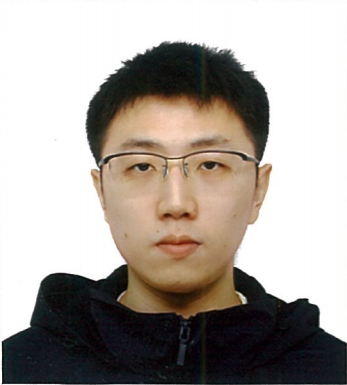
\includegraphics[width=2.8cm]{figure.png}
\end{minipage}

%-----------EDUCATION-----------
\section{教育背景}
\resumeSubHeadingListStart

\resumeSubheading
{早稻田大学}{东京, 日本}
{计算机科学与通信工程专业（基础理工学院）（博士）}{2023.09 -- 2026.09}
\resumeItemListStart
\resumeItem{导师：Prof. Hiroshi Watanabe（\href{https://www.ams.giti.waseda.ac.jp/}{Advance Multimedia Systems(AMS) Lab}）}
\resumeItem{研究方向：多模态目标检测，小目标检测}
\resumeItemListEnd

\resumeSubheading
{早稻田大学}{东京, 日本}
{计算机科学与通信工程专业（基础理工学院）（硕士）（GPA：3.8 / 4.0）}{2021.09 -- 2023.07}
\resumeItemListStart
\resumeItem{导师：Prof. Hiroshi Watanabe（\href{https://www.ams.giti.waseda.ac.jp/}{Advance Multimedia Systems(AMS) Lab}）}
\resumeItem{研究方向：目标检测，行人检测，密集检测}
\resumeItemListEnd

\resumeSubheading
{北京航空航天大学}{北京, 中国}
{信息与计算科学专业（数学科学学院）（本科）（GPA：3.2 / 4.0）}{2016.09 -- 2020.07}
\resumeItemListStart
\resumeItem{核心课程：数理逻辑、最优化理论、概率论、实变/复变函数、泛函分析以及数值分析}
\resumeItemListEnd

\resumeSubheading
{爱尔兰国立梅努斯大学}{梅努斯, 爱尔兰}
{交换项目（核心课程：代数拓扑，微分几何以及偏微分方程）}{2018.09 -- 2018.12}

\resumeSubheading
{伦敦大学学院（UCL）}{伦敦, 英国}
{暑期交流（学术写作）}{2017.07 -- 2017.08}

\resumeSubHeadingListEnd

%-----------RESEARCH INTERESTS-----------
\section{研究兴趣}
\small
\begin{itemize}[leftmargin=0.15in, label={}]
\item \textbf{视觉感知与场景理解：}
面向复杂真实场景的视觉感知问题，包括目标检测、分割与场景图生成，重点关注小目标、密集分布与跨尺度场景下的表征稳定性与泛化能力，并逐步延伸至开放词表检测与语言引导的定位。
% \item \textbf{自监督视觉表征学习：}
% 基于 Transformer 的视觉自监督方法（如 DINO 系列），关注无标注或弱标注条件下语义一致性表征的学习机制，以及其向下游检测与定位任务的迁移。
\item \textbf{多模态视觉感知与跨模态对齐：}
多模态视觉表征学习与跨模态对齐问题，涵盖 RGB–红外/热成像融合、遥感影像理解等感知任务，并进一步关注以多模态大模型（具备开放词表定位能力的轻量级视觉语言模型）为核心的智能体系统，包括视觉–语言联合推理、指代定位、任务规划与工具使用，以及感知结果在下游决策过程中的稳定性与可信性。
\item \textbf{当前工作：}
基于大语言模型的文本到 CAD 生成。通过 LoRA 微调,使模型从自然语言描述直接生成可执行的参数化建模代码(CadQuery),进而得到三维 CAD 模型;并在生成中引入约束以提升结果的有效性。
\end{itemize}
%-----------PUBLICATIONS-----------
\section{学术论文}
{\footnotesize $^{\dagger}$ 为通讯作者}
  \resumeSubHeadingListStart
    \resumeItem{\textbf{Haoyuan Liu}, Hiroshi Watanabe. "InterpIoU: Robust Bounding Box Regression Loss within an Interpolation-Based IoU Framework." \textit{Neurocomputing}, Vol. 666, 2026.}
    
    \resumeItem{\textbf{Haoyuan Liu}, Hiroshi Watanabe. "GSA: Guided Supervised Attention for Enhancing Real-Time Dense Object Detection via Parameter-Free Scheme." \textit{Journal of Electronic Imaging}, Vol. 33(6), Nov. 2024.}

    \resumeItem{\textbf{Haoyuan Liu}, Hiroshi Watanabe. "Feature Transfer Block for Feature Fusion in Lightweight Object Detectors." \textit{IEEE 12th Global Conference on Consumer Electronics (GCCE)}, Oct. 2023.}

    \resumeItem{Ziyue Zeng, Xun Su, \textbf{Haoyuan Liu}, Bingyu Lu, Yui Tatsumi, Hiroshi Watanabe. "GVCC: Zero-Shot Video Compression via Codebook-Driven Stochastic Rectified Flow." \textit{Conference on Neural Information Processing Systems (NeurIPS)}, Dec. 2026. Accepted (Poster).}

    \resumeItem{Bingyu Lu, \textbf{Haoyuan Liu}$^{\dagger}$, Ziyue Zeng, Hiroshi Watanabe. "WMPF: Wavelet-Decoupled Discrepancy Mitigation and Detail-Preserving Fusion for RGB--IR Object Detection." \textit{IEEE/CVF Winter Conference on Applications of Computer Vision (WACV)}, 2027. Accepted (Round 2).}

    \resumeItem{Gaosiheng Chen, Bingyu Lu, \textbf{Haoyuan Liu}, Hiroshi Watanabe. "Partial Cross-Modal Channel Injection for RGB-Infrared Spatial Alignment." \textit{International Workshop on Advanced Image Technology (IWAIT)}, Jan. 2027. Accepted.}

    \resumeItem{Mohan Yin, \textbf{Haoyuan Liu}$^{\dagger}$, Hongrui Fan, Bingyu Lu, Hiroshi Watanabe. "TMSF-YOLO: Two-Round Multi-Scale Fusion with Semantic Feedback for Small-Object Detection." \textit{IEEE International Conference on Systems, Man, and Cybernetics (SMC)}, Bellevue, WA, USA, Oct. 2026. Accepted Jun. 2026.}

    \resumeItem{Bingyu Lu, \textbf{Haoyuan Liu}$^{\dagger}$, Hiroshi Watanabe. "A Foreground-Background Differentiated Fusion Model for RGB-Infrared Object Detection." \textit{IEEE International Conference on Systems, Man, and Cybernetics (SMC)}, Bellevue, WA, USA, Oct. 2026. Accepted Jun. 2026.}

    \resumeItem{Ziyue Zeng, Yupei Guo, \textbf{Haoyuan Liu}, Dingjie Peng, Hiroshi Watanabe. "Time Step Generating: A Universal Synthesized Deepfake Image Detector." \textit{ACM Multimedia Asia (MMAsia)}, Dec. 2025.}

    \resumeItem{Gaosiheng Chen, Bingyu Lu, \textbf{Haoyuan Liu} and Hiroshi Watanabe. "Local Feature Calibration and Adaptive Fusion for Small-Object RGB-Infrared Object Detection" \textit{IEEE GCCE}, Oct. 2026.}

    \resumeItem{Yihua Jing, \textbf{Haoyuan Liu} and Hiroshi Watanabe. "Semantic-Driven Backbone Enhancement for Small Object Detection in UAV Imagery" \textit{IEEE GCCE}, Oct. 2026.}

    \resumeItem{Wotong Li, \textbf{Haoyuan Liu} and Hiroshi Watanabe. "Bridging Gaussian Representation and Real-Time Detection via Cholesky Parameterization" \textit{IEEE GCCE}, Oct. 2026.}

    \resumeItem{Bingyu Lu, \textbf{Haoyuan Liu}, Hiroshi Watanabe. "Enhancing RGB-Infrared Object Detection: A Frozen Backbone Approach with Multi-Receptive Field Attention." \textit{The Visual Computer (Springer Nature)}.}
  
    \resumeItem{Hongrui Fan, \textbf{Haoyuan Liu}, Hiroshi Watanabe. "A Lightweight Channel Bias for Small Object Detection in Aerial Images." \textit{International Workshop on Advanced Image Technology (IWAIT)}, Jan. 2026.}

    \resumeItem{Hongrui Fan, \textbf{Haoyuan Liu}, Hiroshi Watanabe. "Enhancing Object Detection with Non-Local Modules in the Feature Pyramid Network." \textit{IEEE GCCE}, Oct. 2024.}

    \resumeItem{Jiu Yi, \textbf{Haoyuan Liu}, Hiroshi Watanabe. "Distilled RSN: Lightweight Pose Estimation Using Knowledge Distillation." \textit{IEEE GCCE}, Oct. 2024.}
    
    \resumeItem{Jiahao Liu, \textbf{Haoyuan Liu}, Hiroshi Watanabe. "Video Salient Object Detection Using Multi-Scale Self-Attention." \textit{IEEE GCCE}, Oct. 2023.}
  \resumeSubHeadingListEnd

\textbf{在审稿中/准备投稿}
\vspace{-5pt}
  \resumeSubHeadingListStart
    \resumeItem{\textbf{Haoyuan Liu}, Mohan Yin, Bingyu Lu, Wen Yang, Ziyue Zeng, Hiroshi Watanabe. "The Supervision Ceiling: Scale Aware Calibration for Reliable Small Object Detection" Submitted to Pattern Recognition.}

    \resumeItem{\textbf{Haoyuan Liu}, Tianshui Chen, Hiroshi Watanabe, Liang Lin. "Geometry-Adaptive Feature Enhancement and Contextual Diffusion for Small Object Detection in UAV Imagery." Submitted to ISPRS Journal of Photogrammetry and Remote Sensing.}

    % \resumeItem{Bingyu Lu, \textbf{Haoyuan Liu}, Hiroshi Watanabe. "A Foreground-Background Differentiated Fusion Model for RGB-Infrared Object Detection." Under review at \textit{ICASSP 2026}.}

  \resumeSubHeadingListEnd

\section{教学与指导经历}
  \resumeSubHeadingListStart
    \resumeSubheading
      {早稻田大学}{东京, 日本}
      {助教（Teaching Assistant, TA）}{2024.09 -- 2026.09}
      \resumeItemListStart
        \resumeItem{负责讲授 \textit{Multimedia and Standards} 与 \textit{Image Processing} 课程中的部分专题内容与教学模块。}
      \resumeItemListEnd

    \resumeSubheading
      {AMS Lab, 早稻田大学}{东京, 日本}
      {实验室Recognition组会负责人}{2023.09 -- 2026.09}
      \resumeItemListStart
        \resumeItem{负责组会成员（本科生与硕士生）的日常科研指导与研究进度管理。}
      \resumeItemListEnd
  \resumeSubHeadingListEnd

\section{研究经历}
  \resumeSubHeadingListStart

    \resumeSubheading
      {1、香港理工大学}{香港, 中国}
      {\quad 博士后研究员（Lumen Lab）}{2026.10 -- 至今}
      \resumeItemListStart
        \resumeItem{研究方向：基于轻量化语言模型的文本到 CAD 生成、开放词表检测与语言引导定位，以及多模态智能体系统。}
      \resumeItemListEnd
  \vspace{0.2cm}

    \resumeSubheading
      {2、中国电信股份有限公司北京研究院}{北京, 中国}
      {\quad AI研发中心 -- 研究实习生（远程）}{2023.04 -- 2024.12}
      \resumeItemListStart
        \resumeItem{可信AI测评、人工智能合规平台及大模型安全性调研等任务。}
      \resumeItemListEnd
  \vspace{0.2cm}
   \resumeSubheading
    {3、面向鲁棒小目标检测的一阶段检测器多阶段流程优化}{早稻田大学}
    {\quad 博士研究课题}{2023.09 -- 2026.09}
    \resumeItemListStart
    \resumeItemF{小目标检测是目标检测领域长期悬而未决的核心难题。小目标因像素数量极少、特征表征微弱、定位信号不可靠等因素，在检测流程的多个阶段中均面临系统性退化，尤其在无人机航拍等密集场景中表现尤为突出。博士期间，本人以一阶段检测器为平台，围绕小目标在\textbf{特征提取、标签分配与监督优化}三个流程阶段中信号可靠性不足与优化稳定性缺失的问题，系统性地提出了多阶段流程优化方案，形成了一条从特征表征增强、尺度感知匹配到监督信号精炼的完整研究主线。}
  \vspace{0.2cm}
  \resumeItem{\textbf{特征表征增强（投稿中）}：针对标准 CNN-FPN 范式对小目标特征的系统性退化问题，设计\textbf{轻量化局部注意力与上下文感知特征增强框架（CLFE）}，从局部细节保持与跨尺度上下文调控两个维度联合改进特征提取与融合机制，在不明显增加计算开销的前提下显著提升航拍场景下的小目标检测性能。相关成果已发表于 \textit{Journal of Electronic Imaging}（GSA）与 \textit{IEEE GCCE}（FTB），另有工作 \textit{Geometry-Adaptive Feature Enhancement and Contextual Diffusion for Small Object Detection in UAV Imagery} 目前处于期刊评审阶段。}
  \vspace{0.1cm}
  \resumeItem{\textbf{尺度自适应标签分配（准备投稿）}：从训练信号可靠性角度重新审视任务对齐型标签分配方法，揭示固定对齐公式在小目标场景下因定位信号噪声与几何度量不稳定导致的匹配振荡问题，提出一种统一的\textbf{尺度感知动态分配框架（USAA）}，通过难度感知任务权重重调与有界容差几何相似度度量，显著提升小目标正样本匹配的稳定性与一致性。论文 \textit{Unified Scale-Adaptive Label Assignment for Small Object Detection} 目前处于期刊评审阶段。}
  \vspace{0.1cm}
  \resumeItem{\textbf{边框回归损失优化（已发表）}：提出基于插值框架的 \href{https://github.com/NuayHL/interpiou}{\underline{\textbf{InterpIoU Loss}}}，通过在预测框与真值框之间构建连续插值路径，在非重叠及极端几何条件下提供与 IoU 目标严格一致的稳定回归梯度，从根本上消除对手工设计几何惩罚项的依赖，有效缓解小目标定位中的优化不稳定问题。相关成果已发表于 \textit{Neurocomputing}，并被多个后续研究采纳为改进基线。}
\resumeItemListEnd

  \vspace{0.2cm}
\resumeSubheading
{4、单阶段密集行人检测算法}{早稻田大学}
{\quad 硕士研究课题}{2022.04 -- 2023.07}
\resumeItemListStart
  \resumeItem{围绕密集行人场景下单阶段检测器在遮挡干扰与特征冗余条件下检测不稳定的问题，探索多尺度特征融合过程中低开销注意力机制在密集场景中的有效性，提出FTB轻量化注意力方法，用于在多尺度特征融合阶段增强关键行人区域的判别能力。相关方法通过同行评审，被 IEEE 国际会议接收，并提供公开代码实现：\href{https://github.com/NuayHL/CrowdDetection}{\underline{github.com/NuayHL/CrowdDetection}}.}
\resumeItemListEnd

  \vspace{0.2cm}
    \resumeSubheading
      {5、基于卷积神经网络的遥感图像融合}{北京航空航天大学}
      {\quad 本科毕业设计}{2020.02 -- 2020.07}
      \resumeItemListStart
        \resumeItem{基于 ResNet 架构与自监督学习方法，设计卷积神经网络模型解决全色锐化问题，用于高分辨率遥感影像融合。}
      \resumeItemListEnd

  \resumeSubHeadingListEnd


%-----------SKILLS-----------
%\section{技术能力}
%\begin{itemize}[leftmargin=0.15in, label={}]
%\small{
%\item \textbf{编程语言：} Python（熟练），C / C++
%\item \textbf{深度学习相关：} 熟练掌握PyTorch（Custom C++/CUDA Extensions）， Ultralytics（YOLO），MMCV/MMDetection框架。曾独立搭建全流程目标检测训练框架。
%\item \textbf{工具与系统：} Linux，Git，LaTeX，Docker
%}
%\end{itemize}

%\section{获得荣誉}
%  \resumeSubHeadingListStart
%    \resumeProjectHeading
%      {\textbf{国家留学基金委（CSC）公派博士奖学金}}{2023}
%    \resumeProjectHeading
%      {\textbf{美国大学生数学建模竞赛（MCM/ICM）一等奖（Meritorious Winner）}}{2019}
%    \resumeProjectHeading
%      {\textbf{国家留学基金委（CSC）优秀本科生奖学金}}{2018}
%  \resumeSubHeadingListEnd

\end{document}
